\chapter{Simulation et Analyse des résultats}\label{simulation}
%----------------------------------------------------------------------------------------------------------------------------------------------------------
Dans la première partie de ce chapitre, 
nous allons présenter en détail le simulateur conçu pour jouer les diverses politiques concernant les deux fonctions importantes pour une plateforme NUMA, ordonnancer les threads et placer les données. 
Ensuite, plusieurs scenarios d'évaluation des diverses métriques des politiques intégrant les heuristiques proposées sont simulés pour voir l'impact et l'efficacité de cette modification (approches proposées) sur l'exécution des applications parallèles à base de tâches soit indépendantes ou dépendantes (décrites par un DAG). Ensuite une partie complémentaire pour tester l'approche proposée pour équilibrer la charge en utilisant une variante du vol de travail adapté à NUMA.

Dans la section \ref{simHLSM}, nous présentons le simulateur utilisé par la suite et son architec-ture. 
Ensuite, l'expérimentation en combinant les politiques des deux processus ordonnan-cement et placement sur les tâches indépendantes est détaillée dans la section \ref{etiar} suivie par analyse des résultats obtenus pour les scénarios joués.
Dans la section \ref{etdar}, l'expérimentation des heuristiques proposées dans le chapitre précédent sur tâches dépendantes représentés par  DAG au format STG. Les résultats de ces scénarios seront analysés et commentés dans cette même section.   
La dernière idée proposée concernant équilibrage de charge par le vol de travail basé sur la distance et adapté à NUMA est testé dans cette section \ref{eecar} suivie par l'analyse de ces résultats.
Enfin dans la section \ref{conc}, nous concluons ce chapitre.
%====================================================================================
\section{Simulateur NUMA (HLSMN)} \label{simHLSM}
%
La simulation devient un outil important pour l'informatique scientifique pour construi-re et concevoir un modèle avant la phase de production. Les systèmes embarqués et l'architecture informatique deviennent le domaine où cette approche est utilisée de manière intensive pour éviter les problèmes de conception ou pour l'améliorer. 
Les plateformes NUMA sont assez compliquées et diversifiées (architecture, configuration) alors pour concevoir une politique spécifique à cette plateforme et générique à ses variantes et la tester sur plusieurs architectures cible, la simulation est une bonne solution avec un coût acceptable.% \cite{Hager2010}.
%
\subsection{Etat de l'art des simulateurs Multicoeurs NUMA}
%
Plusieurs simulateurs génériques adaptés au système multiprocesseurs et multicoeurs ont été développés. Comme exemple, on peut citer 
Simics, \cite{sim11}, 
GEMS, \cite{GEM12} et 
M5, \cite{M5S13} 
permettant de concevoir et tester ces systèmes avant leur conception concrète et leur production. Des simulateurs dédiés à des architectures spécifiques ont également été développés. Par exemple, des outils pour la mémoire partagée, multicoeurs, manycore et NUMA architecture qui incluent un composant spécifique qui expose les principales fonctionnalités de ces sous systèmes.% \cite{GogFur09OLS}. 

\textbf{RSIM (Rice Simulator for ILP Multiprocessors)}\\  
C'est un simulateur de bas niveau piloté par exécution pour les systèmes multiprocesseurs avec cc-NUMA basé sur un répertoire. 
Il met l'accent sur la précision et il simule un mécanisme de cohérence du cache réseau et un cache basé sur les répertoires. \cite{RSI14, RSI15}.

\textbf{SIMT }\\ %
C'est un outil de simulation pour les machines NUMA qui repose sur un autre outil Augmint \cite{Aug17} 
pour fournir des données de référence de mémoire et se concentre principalement sur la hiérarchie de la mémoire, telles que les erreurs de cache et les invalidations de cache. Il ignore les réseaux d'interconnexion utilisant des constantes comme latences de communication et un temps estimé pour modéliser le temps d'exécution des instructions
\cite{SIM16}.

\textbf{Graphite}\\  %\cite{graphite}
C'est un simulateur parallèle Open Source, distribué pour le laboratoire des architectures multidimensionnelles du MIT, il est conçu de manière à explorer les futurs processeurs multicœurs contenant des dizaines, de centaines, voire des milliers de noyaux. Il est capable d'accélérer les simulations en les distribuant sur plusieurs machines Linux de commodité.
\cite{Gra18}  %\textbf{MCoreSim}\\ Il est conçu pour les manycore et réaliser avec Omnet++.

\textbf{SimNUMA }\\ %17
C'est un simulateur de système complet piloté par exécution dédié aux systèmes d'architec-ture NUMA. Ses principales caractéristiques comprennent: l'utilisation du même type de processeur avec la machine cible dans le système hôte et une nouvelle méthode pour capturer et simuler des accès à la mémoire distante. Il modélise les  différents types de réseaux d'interconnexion. \cite{Sim20}

\textbf{Autres}\\
Il existe des simulateurs plus spécifiques dédiés à un module, une fonctionnalité ou une modélisation de certains aspects de la plate-forme NUMA tel que la simulation de protocole de cohérence de cache ou modélisation de performance. 
SICOSYS \cite{SIC21}
qui est un framework intégré pour évaluer les performances du réseau d'interconnexion. C'est un simulateur de réseau d'interconnexion à usage général. Memphis \cite{Mem22}
est un outil pour trouver et améliorer les problèmes de performance liés à NUMA sur les plateformes multicœur.
  
%
\subsection{Architecture et Conception du simulateur HLSMN}
La plupart des simulateurs cités sont de bas niveau modélisent les éléments de base de ces systèmes et se concentrent sur la structure interne et le processus d'exécution d'instructions en plus de détails (architecture matérielle). 
Cet aspect rend le processus de simulation plus complexe et difficile à manipuler des politiques de haut niveau telles que l'ordonnancement des threads et le placement de données. 
%
\begin{figure}[h]
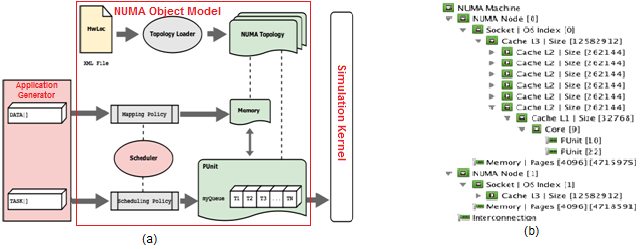
\includegraphics[scale=0.9]{model_sim_numa}
\centering
\caption{NUMA object model structure a- interne b- Arborescence de la topologie}
\label{fig:NUMAMOSIAT}
\end{figure}
%
Un simulateur de haut niveau pour les plateformes multicoeur NUMA (Hihg Level Simulator of Multicore NUMA HLSMN) a été conçu. Sa conception est faite de telle façon qu'elle expose les fonctionnalités de base de la machine MC-NUMA. Sa structure interne est constituée de plusieurs composants interconnectés en fonction de la topologie de la machine cible. Le schéma donné par la figure \ref{fig:NUMAMOSIAT} représente cette conception. 
%\begin{sidewaysfigure}[h]
\begin{figure}[h]
    \centering
    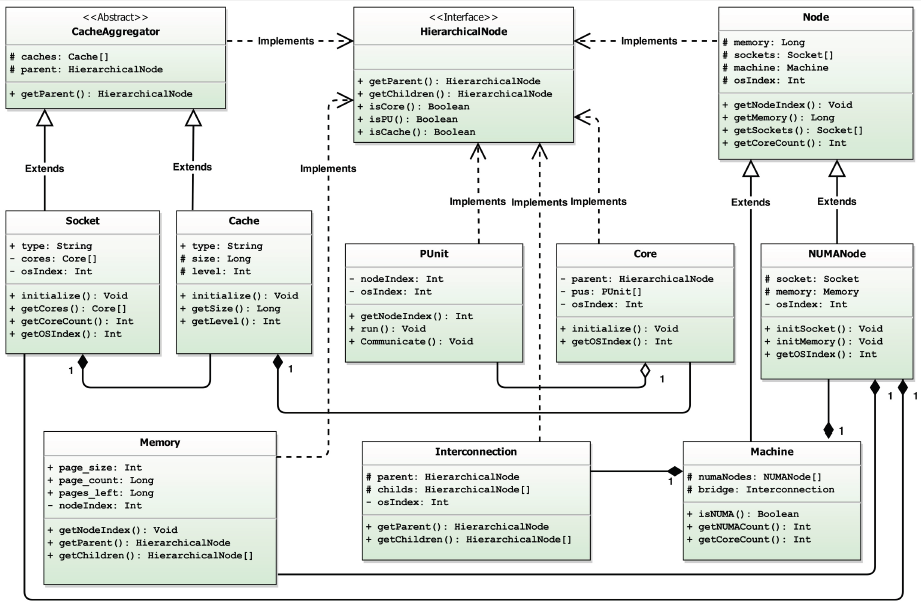
\includegraphics[ scale = 0.65]{om_numa}
    \caption{Architecture du simulateur HLSMN}
    \label{fig:archHLSMN}
\end{figure}
%\end{sidewaysfigure}
\subsubsection{Modèle objet NUMA}
Ce modèle est inspiré de l'outil Xml DTD de Hwloc. Nous effectuons le processus inverse de Hwloc, ces outils génèrent la description basée sur XML d'une plateforme cible réelle à utiliser par l'ordonnanceur. Dans notre cas, nous allons prendre une telle description et construire un modèle d'objet qui correspond à la plateforme cible. La figure \ref{fig:archHLSMN} donne une représentation globale de l'architecture interne de ce simulateur.  Le modèle d'objet se compose de plusieurs modules, y compris:

- \textbf{Machine} : est le module principal à activer pour utiliser le modèle. Il connecte tous les autres modules de manière appropriée en fonction de la description de la topologie.

- \textbf{HierarchicalNode} : est une interface qui résume la structure hiérarchique de cette plateforme. Comme la hiérarchie de la mémoire est structurée comme une arborescence et elle est plus complexe dans NUMA, chaque élément de cette architecture est considéré comme un nœud dans cet arbre (bancs de mémoire, caches, noyau, ...) puis ils partagent les mêmes fonctionnalités d'entités connectées en arbre (accès root ou parent, énumérer la liste de nœuds-fils, notifier la racine ou le parent, ...).

- \textbf{NumaNode} : c'est l'entité la plus importante dans la machine qui modélise l'élément NUMA. Il sera connecté au réseau d'interconnexion et il se comportera seul comme entité SMP.

- \textbf{Socket} : le package processeur contient les unités de calculs (cœurs) et le reste de la hiérarchie mémoire de différents niveaux.

- \textbf{Core} : l'unité de calcul de base qui exécute les threads associés aux tâches d'application.

- \textbf{Interconnexion} : un réseau spécial pour connecter NumaNodes et router les messages entre les différentes entités.

- \textbf{Mémoire} : unités de stockage associées à NumaNode. C'est le stockage local pour ce nœud associé avec une faible latence et une bande passante élevée, contrairement à d'autres nœuds non directement connectés (nœud distant) où la latence est élevée et la bande passante basse.

La figure \ref{fig:archHLSMN} (a) montre les principaux composants de cette partie et expose l'architecture de l'objet NUMA Modèle de HLSMN avec ses composants principaux montrant la relation entre les classes dans le package NUMA. Chaque classe implémente l'interface HierarchicalNode ou étend une autre classe qui l'implémente, de sorte qu'elles héritent des mêmes propriétés et comportements. Sur la base de cette interface, nous pouvons identifier les nœuds-parents et les nœuds-fils dans la hiérarchie en appelant les fonctions getParent() et getChildren() et en récupérant les objets de type HierarchicalNode.
%
\subsubsection{Gestionnaire des topologies}
%
Il est responsable du chargement de la topologie à simuler. Après avoir chargé correctement le fichier associé, il affiche la structure dans la visionneuse de topologie (\ref{fig:archHLSMN} (b)). Ensuite, en fonction de cette structure, il crée le modèle d'objet en instanciant un objet de type Machine et en fait la racine de la hiérarchie. Chaque composant de la topologie possède sa propre classe de représentation qui est initialisée et qui invoque une autre méthode pour créer des sous-éléments ou des enfants dans cet ordre:
%
\subsubsection{Générateur de l'application}
%
Pour exécuter différents scénarios de simulation, nous avons conçu un générateur des applications modèles (Template). Sa tâche consiste à générer des tâches aléatoires en fonction du modèle donné. Le modèle d'application se compose de tâches définies avec des caractéristiques de calcul et la communication doit représenter une classe d'applications parallèles réelles qui partagent un certain profil (application avec plus de calcul et moins de communication ou communication intense) et spécifie les données et le volume nécessaire pendant l'exécution. Selon ce modèle, ce module générera une instance d'application à transmettre comme paramètre au modèle d'objet.
%
\subsubsection{Noyau de simulation}  %\textbf{Exécuteur des politiques}
%
Ce module est le cœur du simulateur. C'est le noyau qui est responsable de la gestion des processus de simulation, de la synchronisation des événements et de la communication entre les entités de simulation. Lors du démarrage du simulateur et après le chargement de la topologie et de la génération de tâches / données (instance), le module de configuration obtient divers types de paramètres sur la machine cible à partir du modèle d'objet, tel que le nombre de processeurs, la taille de la mémoire, les paramètres d'interconnexion tels que le type, la topologie, la bande passante, la politique de routage, etc. et la structure et les détails de l'instance d'application. Ce module essaie de jouer une politique d'ordonnancement choisie sur l'instance donnée de l'application pour prendre les décisions concernant le temps début d'exécution et les nœuds alloués. Ensuite, il mappe les données associées sur les mémoires de nœud en utilisant une autre politique de placement de données choisie. Enfin et lorsque les tâches sont prêtes à être exécutées sur la ressource disponible, l'exécution est lancée sur le nœud alloué et en affectant les données à la mémoire choisie. Il est basé sur la capture des événements survenus sur chaque objet du modèle d'objet, le renvoi et la notification des parties intéressées aux événements survenus. À mesure que les modules fonctionnent simultanément dans ses threads de travail (cœurs, mémoires, interconnexions), il assure la synchronisation et la communication entre eux pour accéder aux ressources partagées (événements de file d'attente, ...).

Comme il est important et critique dans le processus de simulation de garder l'historique, nous avons conçu avec le simulateur, un outil pour enregistrer la trace de la simulation et en collectant les statistiques. 
%====================================================================================
\newpage
\section{Expérimentation tâches indépendantes} \label{etiar}
%
Le scénario de simulation spécifique consiste à configurer les paramètres de l'enviro-nnement de simulation en spécifiant la topologie cible, le modèle d'application pour créer une instance, en choisissant les stratégies d'ordonnancement et de placement à appliquer sur les tâches et les données. Ensuite, nous lançons l'expérimentation en utilisant les paramètres spécifiés. Enfin, nous recueillons les résultats de cette simulation en enregistrant les événements. La dernière étape consiste à analyser les résultats obtenus.
%
\subsection{Configuration de la simulation}
%
Cette étape consiste à définir les informations de configuration utilisées lors du processus de simulation. En combinant les différentes valeurs des paramètres, la configuration obtenue correspond à un scénario d'expérimentation par la suite. Les paramètres les plus importants sont:

- \textbf{Topologie cible}: est définie via le chargeur de topologie en fournissant le fichier de configuration XML de cette topologie.

- \textbf{Modèle d'application}: il est spécifié dans le générateur d'application en donnant le profil de l'application soumise. Ce générateur crée une instance avec le nombre spécifié de tâches avec des données privées prédéfinies et selon le profil spécifié.

- \textbf{Politique ordonnancement/placement}: spécifier quelle stratégie à utiliser pour l'exécution en fonction des politiques/heuristiques implémentées (à évaluer et à tester).
%
\subsection{Expérimentation des scénarios}
%
Dans cette section, nous aborderons le processus d'expérimentation et d'évaluation de certains scénarios de simulation. Le scénario de simulation avec la topologie cible, le modèle d'application des tâches indépendantes de grains de taille moyenne avec moins de communication (opérations de données Read / Write faibles) et l'ordonnancement de type X avec Y comme stratégie de placement représente une expérience qui va mesurer l'impact de combiner ces deux stratégies sur la classe de l'application choisie. Aux fins de cette expérimentation, nous avons mis en œuvre :\\
- \textbf{Politiques d'ordonnancement} : \textit{Round Robin (SRR)} et \textit{Load Balanced (SLL)}\\
- \textbf{Stratégies de placement}: \textit{First Touch (PFT)} et \textit{Round Robin Allocation (PRR)}

Notre expérience consiste à tester toutes les politiques possibles d'ordonnancement et placement combinées avec deux modèles d'application \textbf{T50} et \textbf{T250} (la première contient 50 tâches indépendantes avec ses 50 données associées et la seconde avec 250) cela nous donnera 8 différents scénarios \textbf{[SRR, SLB] $\times$ [PRR, PFT] $\times$ [T50, T250]}. Et, par conséquent, nous sommes intéressés par le temps d'exécution total et le nombre d'accès distant dans chaque scénario.
%
\subsection{Analyse des Résultats}
%
Nous présentons ici la moyenne des résultats après la répétition des expériences qui correspondent à chaque scénario. D’abord une première expérimentation concernant la métrique temps total d'exécution et puis nous montrerons une deuxième mesurant la pénalité NUMA. 
%Lorsque l’on lance les programmes de test, nous obtenons la courbe et le schéma donnés dans les figures 4.5, 4.6 et 4.7.

Le tableau \ref{table:TotalExeTimeSCAB00} donne le temps total d'exécution pour chaque scenario qui est graphique-ment représenté par La figure \ref{fig:TotalExeTimeSCAB}.

Dans les scenarios de 50 tâches, les scenarios configurés avec le placement PFT (6.18, 7.213) donnent un temps total d'exécution meilleur que celui du PRR (7.854, 11.372). Dans les scenarios de 250 tâches, toujours le placement PFT (21.877, 39.084) présente des meilleurs résultats par rapport à l'autre stratégie PRR (25.799, 40.107). En comparant cette fois par rapport à la stratégie d'ordonnancement, nous observons que la politique SRR n'a pas pu dépasser sa concurrente en donnant un temps total d'exécution (25.799, 40.107) nettement supérieur à celui de SLL (21.877, 39.084). 

Le fait de mapper les données d'une tâche selon la stratégie PFT (sur la mémoire du nœud sur lequel elle tourne), cette décision a influencé son temps total d'exécution par rapport PRR (de distribuer les données à tour de rôle sur les mémoires des nœuds de la plateforme). Cela est peut-être dû à un nombre d'accès moins important que celui de PRR puisque chaque tâche charge ses données dans sa mémoire locale si elle est la première à y accéder. Alors ce facteur a réduit la communication distante donc il a permis de terminer tôt la tâche et en conséquence  de donner un temps total d'exécution inférieur par rapport la distribution RR qui ne tient pas en compte la source de la requête d'allocation mémoire (quelle tâche a demandé cette donnée\?). C'est pourquoi il va générer plus de communication distante donc retarder la terminaison de la tâche et donner un $C_{max}$ important.
%
\begin{table}[h!]
\centering
\begin{tabular}{| c | c | c | c | c |} 
\hline
Tasks/Policy	& PRR-SRR 	& PRR-SLL 	& PFT-SRR 	& PFT-SLL 	\\ [0.5ex] \hline
50 Tasks 		& 7.854 		& 11.372 		& 6.18			& 7.213 		\\ [0.5ex] \hline
250 Tasks		& 25.799 		& 40.107 		& 21.877 		& 39.084 		\\ [0.5ex] \hline
\hline
\end{tabular}
\caption{Temps total d'exécution de chaque scénario 50/250 tâches}
\label{table:TotalExeTimeSCAB00}
\end{table}

La figure \ref{fig:RemoteAccessMemTraceAB} montre graphiquement les accès distants aux données effectués par les tâches résidants sur les nœuds de la plateforme. Comme prévu, Les 50 tâches ont un nombre d'accès distants moins important que les 250 tâches. En comparant maintenant entre les stratégies testées, le nombre des accès distant pour PRR-SRR et PFT-SRR est nettement inferieurs (moins de lignes colorées) à celui de PRR-SLL et PFT-SLL pour les deux scénarios. (La densité des lignes en vert et rouge est faible par rapport la densité des lignes en bleu et jaune). 

Ce scénario a donné un résultat qui n'était pas prévu puisque la politique PFT s'est comportée comme l'autre politique PRR en générant un nombre similaire d'accès distant malgré qu'elle charge les données dans la mémoire locale de la tâche demandeuse. Une interprétation possible est qu'il y a assez de tâches qui partagent la même donnée et puisque il n'y a pas de  migration de tâche alors la première qui demande la donnée elle l'obtient en local mais le reste doit faire une communication distante pour l'utiliser (en lecture ou écriture).

%
\begin{figure}[h]
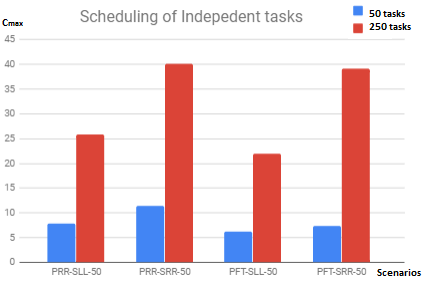
\includegraphics[scale=0.9]{result_numa022}
\centering
\caption{Temps total d'exécution pour chaque scénario (a) 50 tâches (b) 200 tâches}
\label{fig:TotalExeTimeSCAB}
\end{figure}
%
\begin{figure}[h]
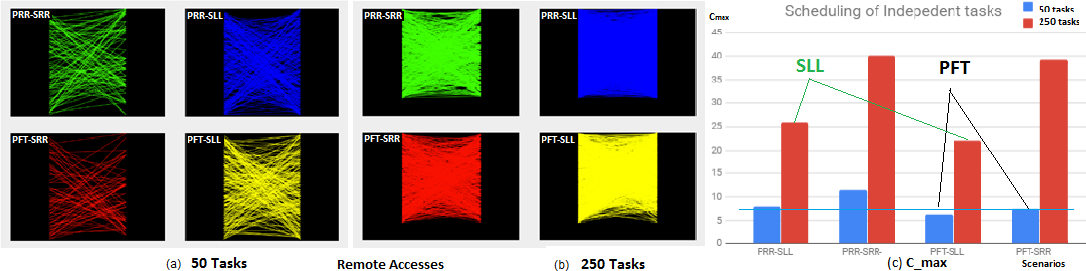
\includegraphics[scale=0.80]{result_numa01}
\centering
\caption{Trace des acces mémoire distants (a) 50 tâches (b) 200 tâches}
\label{fig:RemoteAccessMemTraceAB}
\end{figure}
%

%
%====================================================================================
\newpage
\section{Expérimentation tâches dépendantes DAG} \label{etdar} 
%
Dans cette section nous allons expérimenter notre heuristique. Tout d'abord, un scenario d'expérimentation sur des applications parallèles de différente configuration (DAGs dont le nombre de tâches et structures différentes) est réalisé en mesurant le temps total d'exécution sur des plateformes NUMA de différentes architectures. Ensuite le même scenario d'expérimentation est répété pour les même applications parallèles mais cette fois on s'intéresse à la pénalité NUMA.
%
\subsection{Configuration de la simulation}
%
Afin de configurer les scénarios de simulation, nous présentons les différentes rubriques et les options à paramétrer :\\
\textbf{Topologie simulée} :\\
- \textit{Plateforme configuration Nombre de nœuds/cœurs (xNyC)}\\
- \textit{Réseaux ICN} : La matrice des distances entre les nœuds est donnée comme paramètre de simulation.
\\
\textbf{Jeu de Test} \\
Ce jeu de test est choisi parmi l'ensemble des DAGs au \textbf{format STG} \cite{STG16} qui constitue une référence pour le test des problèmes utilisant des DAGs. Le format STG a été enrichi en ajoutant un champ appelé motif d'accès mémoire spécifique pour les architectures NUMA. Le listing suivant donne un exemple d'un DAG codé en STG avec l'extension motif d'accès. La notation utilisée est DAGXx ou Xx est le nombre de tâches du DAG utilisé (DAG50 contient 50 tâches).
%
\begin{Verbatim}[formatcom=\color{blue}]
//DAG050 au format STG de 50 Tâches et avec sa précédence
	50
	00	00	0	-	S;0;20;R;1;50;W;0;30;E;1;0
	01	09	1	0	S;2;30;R;3;20;W;2;50;E;3;0
	02	04	1	0	S;4;50;R;5;30;W;4;20;E;5;0
	03	03	1	0	S;6;20;R;7;50;W;6;30;E;7;0
	04	06	1	0	S;0;20;R;1;50;W;0;30;E;1;0
	05	04	1	1	S;2;30;R;3;20;W;2;50;E;3;0
	06	03	1	5	S;4;50;R;5;30;W;4;20;E;5;0
	07	03	1	0	S;6;20;R;7;50;W;6;30;E;7;0
	08	08	1	6	S;0;20;R;1;50;W;0;30;E;1;0
	09	09	1	0	S;2;30;R;3;20;W;2;50;E;3;0
	10	02	3	2;6;8  S;4;50;R;5;30;W;4;20;E;5;0
	11	01	1	9	S;6;20;R;7;50;W;6;30;E;7;0
	12	10	1	0	S;0;20;R;1;50;W;0;30;E;1;0
........
\end{Verbatim}
%
\begin{table}[h!]
\centering
\begin{tabular}{| c | c | c | c | c |} 
\hline
Task.id 		& Length 	& Number of Prec 	& Precedences 	& Task Data access pattern \\ [0.5ex] \hline
10 			& 2 	& 3 		& 2;6;8 		& S;4;50;R;5;30;W;4;20;E;5;0 \\ [0.5ex] \hline
\end{tabular}
\caption{Ligne tâche dans le fichier DAG au format STG étendu}
\label{table:TB_2_22220}
\end{table}
%
Le DAG décrit par ce fichier a 50 tâches dont la tâche 0 est la \textbf{tâche d'entrée}, chaque ligne contient l'\textbf{identifiant} de la tâche, sa \textbf{longueur}, le \textbf{nombre de ses prédécesseurs}, la \textbf{liste de ses prédécesseurs} et à la fin le champ supplémentaire pour le cas de NUMA ou en spécifiant le \textbf{motifs d'accès} aux données. Ce motif décrit le schéma d'exécution de sa tâche, il commence avec \textbf{S (start)} en spécifiant les données à charger ou lancement de la tâche ensuite le pourcentage des instructions exécuter par le cœur par rapport au nombre total des instructions de la tâche suivi par une communication soit \textbf{lecture (READ/LOAD)} ou \textbf{écriture (WRITE/STORE)} en spécifiant la donnée concernée et enfin l'étape de la finalisation \textbf{E (end)} de l'exécution de la tâche en sauvegardant les données avant sa terminaison.
\\
\textbf{Heuristiques simulés Ordonnancement}\\   %- \textbf{UMA}   : sur la plateforme UMA \\
- \textit{NXH}   : sur la plateforme NUMA sans Horizon d'exécution \\
- \textit{WXH}  : sur la plateforme NUMA avec l'heuristique Horizon d'exécution X-VHFU
\\
\textbf{Placement}\\
- \textit{AoFT} : Affinity-on-First-Touch
\\
\textbf{Métriques mesurées}\\  %- \textbf{NR} : NUMA ratio\\
- \textit{Cmax} : Temps Total d'exécution\\
- \textit{NR} : Penalité NUMA
%--------------------------------------------------------------------------------
\subsection{Expérimentation des scénarios}
%
Nous allons réaliser deux scénarios qui ont la même configuration d'expérimentation. L'objectif visé dans le premier est de mesurer le temps total d'exécution et dans le deuxième sera la pénalité NUMA.\\
%
\textbf{Scenario 01} :\\
La configuration de ce scénario est la suivante : \\
- \textbf{PF} : 8N2C, 4N4C, 8N1C, 4N2C, 2N4C, 2N2C\\
- \textbf{DAG} : DAG25, DAG50, DAG75, DAG100, DAG125, DAG150\\
- \textbf{S/P} : NXH, WXH / AoFT\\
- \textbf{Métrique mesurée} : Temps Total d'exécution\\
%
\textbf{Scenario 02} :\\
La configuration de ce scénario est la suivante : \\
- \textbf{PF} : 8N2C, 4N4C, 8N1C, 4N2C, 2N4C, 2N2C\\
- \textbf{DAG} : DAG25, DAG50, DAG75, DAG100, DAG125, DAG150\\
- \textbf{S/P} : NXH, WXH / AoFT\\
- \textbf{Métrique mesurée} : Penalité NUMA\\
%
\subsection{Analyse des Résultats}
%
\textbf{Scenario 01} :\\
%
La figure \ref{fig:fig100400x} donne un exemple d'une expérience effectuée en exécutant un DAG STG de 100 tâches sur une plateforme de 4 nœuds et 2 cœurs sur chaque nœuds. La figure représente le diagramme de GANT de l'exécution des tâches sur les cœurs ($P_i$) des nœuds de la plateforme. Nous pouvons voir l'affectation de chaque tâche, sa date début d'exécution, sa fin d'exécution et son temps d'exécution. Les contraintes de précédence imposent la précédence et une synchronisation entre les tâches dépendantes (tâches filles et mères) qui se manifestent comme un temps d'attente (de communication inter tâches $C_i$) de la terminaison des tâches précédentes pour lancer une tâche fille. $C_{max}$ est le temps maximum enregistré par la dernière tâche du DAG pour finir.
%
\begin{figure}[h!]
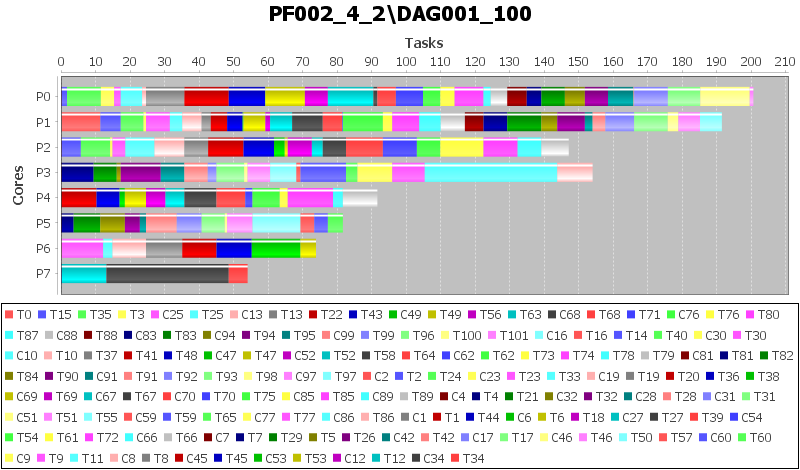
\includegraphics[scale=0.75]{dag1004}
\centering
\caption{Diagramme GANT résultat de l'exécution d'un scénario}
\label{fig:fig100400x}
\end{figure}
%
%
\begin{figure}[h!]
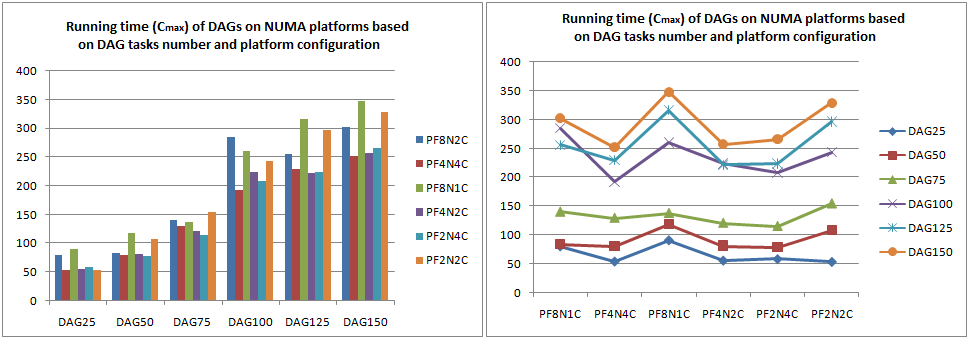
\includegraphics[scale=0.60]{STATISPHD001}
\centering
\caption{Scénario d'expérimentation pour mesurer $C_{max}$}
\label{fig:fg10200x}
\end{figure}
%
La figure \ref{fig:fg10200x} donne le $C_{max}$ associé à chaque DAG ordonnancé sur la plateforme cible. Il montre que pour les DAGs qui ont plus de 100 tâches le $C_{max}$ dépasse 200 unité temps sur toute les plateformes. Mais pour les DAGs dont le nombre de tâches est inferieur à 75 cette valeur reste au dessous de 150 unités temps sur les plateformes testées.

Dans ce premier scénario, Les statistiques collectées concernent le temps total d'exécution en fonction de la politique utilisée pour ordonnancer les tâches (en utilisant l'heuristique XH-VHFU ou non). La stratégie XH est basé sur le principe de la sélection de la tâche à exécuter qui va élargir l'horizon d'exécution après sa sélection, par contre la stratégie classique sélectionne la première qui est en-tête de la liste de tâches prêtes.

La figure \ref{fig:fig1045} donne les détails de l'expérimentation du scénario courant dont la métrique mesurée est le temps total d'exécution pour l'ensemble des DAGs pour les deux cas avec activation XH ou non. En fonction de chaque DAG, \\
\\
- DAG25 : 4 cas sur 6 que les tests avec XH activé dépassent ceux sans XH avec une moyenne d'écart de 4 \% et les valeurs des deux tests s'étalent sur la plage 55 à 88.\\
- DAG50 : 5 cas sur 6 que les tests avec XH activé dépassent ceux sans XH avec une moyenne d'écart de 6 \% et les valeurs des deux tests s'étalent sur la plage 75 à 112.\\
- DAG75 : 5 cas sur 6 que les tests avec XH activé donnent des valeurs supérieures aux valeurs du tests ans XH avec une moyenne d'écart de 7\% et les valeurs des deux tests s'étalent sur la plage 110 à 180.\\
- DAG100 : 5 cas sur 6 que les tests sans XH activé dépassent ceux avec XH avec un écart faible dont la moyenne est -3 \% et les valeurs des deux tests s'étalent sur la plage 190 à 290.\\
- DAG125 : 5 cas sur 6 que les tests avec XH activé dépassent ceux sans XH avec une moyenne d'écart de 4\% et les valeurs des deux tests s'étalent sur la plage 215 à 355.\\
- DAG150 : 4 cas sur 6 que les tests avec XH activé dépassent ceux sans XH avec une moyenne d'écart de 3 \% et les valeurs des deux tests s'étalent sur la plage 255 à 360.

%\begin{table}%[h!]
%\centering
%\begin{tabular}{| c | c | c | c | c | c | c |} 
%\hline
%DAG/PF 	& PF8N2C 	& PF4N4C 	& PF8N1C 	& PF4N2C 	& PF2N4C  	& PF2N2C \\ [0.5ex] \hline
%25 		& 80.35 	& 54.24 		& 90.83 		& 55.67 		& 58.34  		& 53.49 \\ [0.5ex] \hline
%50 		& 83.43 	& 80.39 		& 117.93 		& 81.07 		& 79.04  		& 107.76 \\ [0.5ex] \hline
%75 		& 140.37 		& 129.72 		& 138.17 		& 120.98 		& 115.25  		& 154.95 \\ [0.5ex] \hline
%100		& 285.25 		& 192.37 		& 260.72 		& 224.07 		& 208.67  		& 243.54 \\ [0.5ex] \hline
%125		& 256.38 		& 229.93 		& 316.39 		& 222.07 		& 224.43  		& 296.56 \\ [0.5ex] \hline
%150		& 802.53 		& 251.84 		& 348.24 		& 257.11 		& 265.26  		& 328.80 \\ [0.5ex] \hline
%\hline
%\end{tabular}
%\caption{charge moyenne de la plateforme NUMA x3}
%\label{table:TB_2_1}
%\end{table}
%
Les résultats présentés montrent que l'intégration de heuristique XH a donnée dans la plupart des cas (en moyenne 4 cas sur 6) des écart positif en améliorant le temps total d’exécution entre 3\% à 6\% en moyenne par rapport à la stratégie normale. La découverte de l'horizon au fur et a mesure de l'avancement du processus de l'ordonnancement permet de guider le processus de la prise de décision pour sélectionner la tâches courante à exécuter en exploitant les informations de la visibilité des tâches non encore exécutées en récompensant le manque de l'information concernant la longueur de tâches et les données et le volume échangés entre les tâches.\\
%
\afterpage{
\clearpage 
\thispagestyle{empty}
\begin{landscape}
\begin{center}

\begin{figure}[h!]
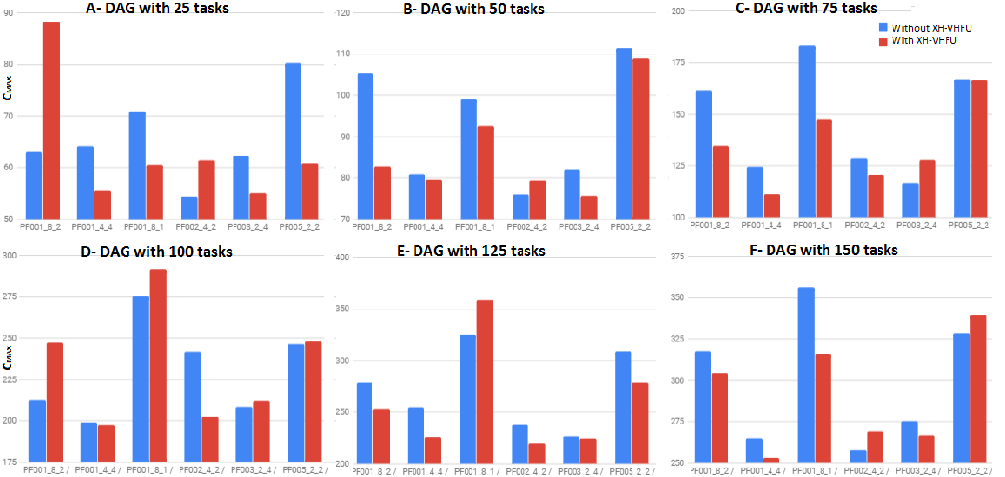
\includegraphics[scale=0.75]{hx002-00}
\centering
\caption{Temps total d'exécution mesuré pour le scénario joué}
\label{fig:fig1045}
\end{figure}

\end{center} 
\end{landscape}
\clearpage
}
%\newpage
\textbf{Scenario 02} :\\
Dans ce deuxième scénario, Les statistiques collectées concernent la pénalité NUMA (le rapport entre le nombre des accès distants par rapport  le nombre des accès locaux, nous allons utiliser un facteur équivalent le pourcentage des accès distants par rapport au nombre total d'accès) en fonction de la politique utilisée pour ordonnancer les tâches (en utilisant l'heuristique XH-VHFU ou non). Lors de l'exécution du code d'une tâche, si l'instruction exécutée est un chargement/une sauvegarde (LOAD/STORE) alors une requête qui correspond à cette opération est faite au système mémoire si la donnée sollicitée est sauvegardé dans la mémoire du nœud exécutant sa tâche alors c'est accès local. Le cœur exécutant adresse cette requête au contrôleur mémoire local qui se charge de récupérer la donnée. Par contre si l'emplacement est sur une mémoire distante alors l'accès est distant. 

Le tableau \ref{table:TB_2_2222} donne le nombre des accès locaux et distants pour l'ensemble des DAGs testés et les valeurs de la pénalité associées pour la première option sans l'utilisation de l'heuristique proposée. Pour la plateforme PF2N2C, la plage des valeurs enregistrées est entre 74\% et 79\%.  Le deuxième tableau \ref{table:TB_2_2223} utilise le même paramètre sauf que cette fois la politique configurée est l'heuristique XH-VHFU. Pour la même plateforme PF2N2C, la plage des valeurs enregistrée est entre 70\% et 78\%. 
Dans les deux cas, le nombre des accès distants dépasse 70\% qui est un pourcentage élevé et un indicateur d'une mauvaise localité malgré l'utilisation de la stratégie AoFT. La deuxième série de tests (avec heuristique) a relativement des valeurs inferieures à par rapport à la première série (sans heuristique), mais cette amélioration est minime et n'est pas significative pour réduire l'impact de cette pénalité sur la performance système.

La figure \ref{fig:fig10450} donne Les détails de l'expérimentation du scénario courant dont la métrique mesurée est la pénalité NUMA pour l'ensemble des DAGs pour les deux cas avec activation XH ou non. En fonction de chaque plateforme, \\
\\
- PF2N2C : 5 cas sur 6 que les tests avec XH activé dépassent ceux sans XH avec une moyenne d'écart de 4 \% et les valeurs des deux tests s'étalent sur la plage 70\% à 78\%.\\
- PF2N4C : 4 cas sur 6 que les tests avec XH activé dépassent ceux sans XH avec une moyenne d'écart de 2 \% et les valeurs des deux tests s'étalent sur la plage 80\% à 89\%.\\
- PF4N2C : 4 cas sur 6 que les tests avec XH activé donnent des valeurs légèrement supérieure aux valeurs du tests ans XH avec une moyenne d'écart de -2 \%  car les deux autre cas présentent un écart important et les valeurs des deux tests s'étalent sur la plage 80\% à 89\%.\\
- PF8N2C 3 cas sur 6 que les tests sans XH activé dépasse ceux avec XH avec un écart remarquable dont la moyenne est -3 \% et les valeurs des deux tests s'étalent sur la plage 82\% à 92\%.\\
- PF8N1C 3 cas sur 6 que les tests avec XH activé dépassent ceux sans XH avec une moyenne d'écart de 2 \% et les valeurs des deux tests s'étalent sur la plage 82\% à 89\%.\\
- PF4N4C 3 cas sur 6 que les tests avec XH activé dépassent ceux sans XH avec une moyenne d'écart de 1 \% et les valeurs des deux tests s'étalent sur la plage 82\% à 91\%.

Les résultats présentés montrent que l'impact de l'intégration de heuristique XH n'a pas été significatif pour réduire le nombre d'accès distant  certes dans 4 tests sur 6 elle a contribué à réduire cette pénalité mais cette réduction n'est pas suffisante vu que la plage des valeurs reste très importante et l'écart trouvé relativement faible. 
%
\begin{table}%[h!]
\centering
\begin{tabular}{| c | c | c | c | c | c | c |} 
\hline
Access 		& DAG25 	& DAG50 	& DAG75 	& DAG100 	& DAG125  	& DAG150 \\ [0.5ex] \hline
Local 			& 25 	& 54 		& 64 		& 108 		& 110  		& 161 \\ [0.5ex] \hline
Remote 		& 83 	& 154 		& 243 		& 300 		& 398  		& 447 \\ [0.5ex] \hline
Rate 		& 77 		& 74 		& 79 		& 74 		& 78  		& 74 \\ [0.5ex] \hline
\hline
\end{tabular}
\caption{Pénalité NUMA pour chaque instance DAG sans XH-VHFU}
\label{table:TB_2_2222}
\end{table}

\begin{table}%[h!]
\centering
\begin{tabular}{| c | c | c | c | c | c | c |} 
\hline
Access 		& DAG25 	& DAG50 	& DAG75 	& DAG100 	& DAG125  	& DAG150 \\ [0.5ex] \hline
Local 			& 28 	& 62 		& 74 		& 101 		& 139  		& 167 \\ [0.5ex] \hline
Remote 		& 80 	& 146 		& 234 		& 307 		& 369  		& 441 \\ [0.5ex] \hline
Rate 		& 74 		& 70 		& 76 		& 75 		& 73  		& 73 \\ [0.5ex] \hline
\hline
\end{tabular}
\caption{Pénalité NUMA pour chaque instance DAG avec XH-VHFU}
\label{table:TB_2_2223}
\end{table}
%
\afterpage{
\clearpage
\thispagestyle{empty}
\begin{landscape}
\begin{center}

\begin{figure}[h!]
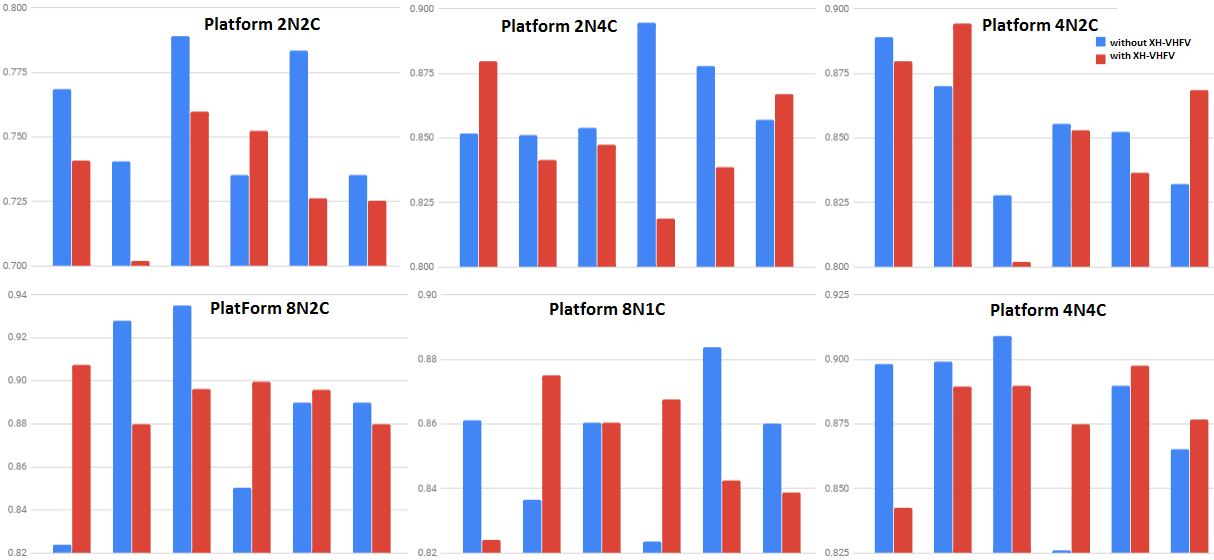
\includegraphics[scale=0.75]{rla_00}
\centering
\caption{Pénalité NUMA mesuré pour scénario joué}
\label{fig:fig10450}
\end{figure}

\end{center} 
\end{landscape}
\clearpage
}   
%====================================================================================
\newpage
\section{Expérimentation Equilibrage de charge} \label{eecar}
%
Dans cette section nous allons expérimenter notre heuristique concernant l'équilib-rage de charge lors de l'exécution des tâches sur une plateforme NUMA. Dans un premier temps, un scenario d'expérimentation configuré sans option d'équilibrage de charge. Dans ce scénario, une série de tâches est lancée sur une plateforme NUMA et durant le déroulem-ent de l'exécution nous allons collecter l'information sur la charge courante sur chaque nœud à la fin nous calculons la charge moyenne sur le système. Un deuxième scénario est configuré avec l'activation de l'option de l'équilibrage de charge en utilisant la stratégie proposée dans de cette thèse à savoir le vol de travail basé sur la distance et adapté à l'architecture NUMA.%
\subsection{Configuration de la simulation}%
La configuration simulée est la suivante :\\
- \textbf{Topologie simulée} : Plateforme configuration Nombre de nœuds/cœurs (4N1C)\\  %8N2C, 4N4C, 8N1C, 4N2C, 2N4C, 2N2C\\
- \textbf{Jeu de Test} : Une série de 1500 tâches\\
- \textbf{Heuristiques simulés Equilibrage de charge} : sans /avec vol de travail basé sur la distance\\
- \textbf{Métriques mesurées} : La charge moyenne\\  %- \textbf{NR} : NUMA ratio\\
%--------------------------------------------------------------------------------
\subsection{Expérimentation des scénarios}
%
\textbf{Scenario 01} 

Dans ce scenario, l'expérimentation est faite sur une plateforme NUMA de quatre nœuds et un cœur pour chaque nœud avec 1500 tâches indépendantes en la paramétrant sans ou avec une stratégie de l'équilibrage de charge.  Pour cette stratégie, nous avons testé dreux variantes basées sur le vol de travail celle la classique (dont la sélection des victimes est aléatoire) et celle l'adaptée à NUMA basée sur la distance. Le but de cette expérimentation est d'évaluer la charge instantanée au cours de l'exécution et sa charge moyenne.\\
1- Topologie simulée : \textbf{4N1C}\\
2- Jeu de Test : \textbf{1500 tâches}\\
3- Heuristiques simulés Equilibrage de charge : sans ou avec vol de travail (\textbf{NWS}, \textbf{WWS})\\ 
4- Métriques mesurées : \textbf{AL} la charge moyenne

Une série de test sur 1500 tâches est lancée en mesurant instantanément la charge sur chaque nœud de la plateforme et à la fin 
nous calculons la charge moyenne. 

Dans un premier temps, la stratégie de l'équilibrage de charge est désactivée. \\
- Heuristiques simulés Equilibrage de charge : - \textbf{NLB} sans vol de travail

Ensuite un deuxième lot de test avec la même configuration est lancé en utilisant le vol de travail classique pour équilibrer la charge. \\
- Heuristiques simulés Equilibrage de charge : - \textbf{CWS} avec vol de travail classique\\

Enfin un troisième lot de test avec la même configuration est lancé mais cette fois en activant l'équilibrage de charge utilisant l'heuristique vol de travail basée sur la distance adaptée à NUMA. \\
3- Heuristiques simulés Equilibrage de charge : - \textbf{dbANWS} avec vol de travail Adapté NUMA basé sur la distance\\

L'évolution de la charge instantanée sur les nœuds correspond à ce scénario est présentée par la figure \ref{fig:xws01}. Le cas A représente le scénario sans l'utilisation du vol de travail et le cas B active cette option la variante basé sur la distance adaptée NUMA. 
%
\begin{figure} %[h!]
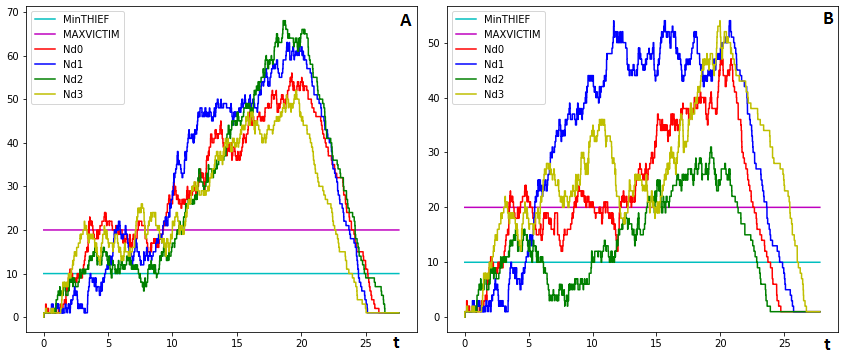
\includegraphics[scale=0.70]{xws01}
\centering
\caption{Charge instantanée des nœuds avec/sans vol de travail adapté NUMA}
\label{fig:xws01}
\end{figure}
%
\subsection{Analyse des Résultats}
%
La figure \ref{fig:fg101} représente l'évolution de la charge moyenne des nœuds de la plateforme NUMA. La partie A concerne les tests sans équilibrer la charge. Dans la partie B, le vol de travail classique est utilisé comme stratégie pour équilibrer la charge, et la dernière partie C, nous avons remplacé la stratégie vol de travail classique par notre variante adaptée NUMA.   
%
\begin{figure}[h!]
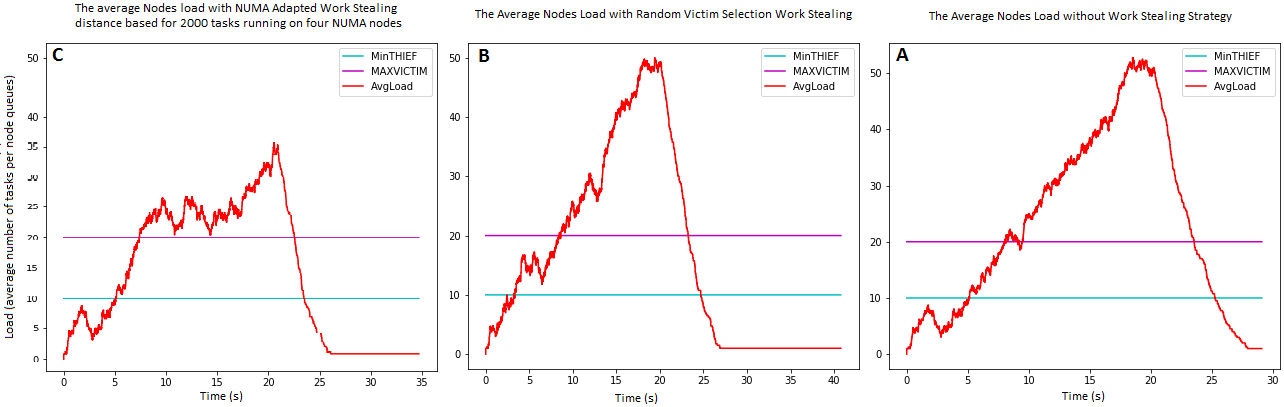
\includegraphics[scale=0.45]{myfigs9-f}
\centering
\caption{Charge moyenne de la plateforme NUMA 4 noeuds}
\label{fig:fg101}
\end{figure}
%
\\
Dans ce scénario, les statistiques collectées concernent la charge sur les noeuds en fonction de la politique d'équilibrage de charge  utilisée (sans vol de travail, avec vol travail aléatoire et avec vol travail adapté NUMA). Apres la soumission d'un lot de taches à un ordonnanceur à exécuter, nous avons enregistré la charge instantanée sur chaque noeud. Selon la figure \ref{fig:xws01}, l'évolution de la charge sur les noeuds s'est accelérée pour atteindre un pic maximum de 70 taches et un pic minimum de 50 taches pour le cas sans utilisation de vol de travail. Par contre, lorsque nous avons activé cette option un pic maximum 52 taches et minimum de 28 taches ont été enregistré. Nous constatons que cette option a redistribué la charge de la plateforme en évitant une surcharge sur les noeuds au meme moment. La figure \ref{fig:fg101} montre que les charges moyennes enregistrées avec les deux premieres strategies sont presque similaires dont l'évolution est croissante jusqu'à un pic maximum de 50 taches. Par contre, la stratégie vol de travail basé sur la distance a donné une charge moyenne plus stable et beaucoup plus inferieure que la précedente. Avec un pic de 35 taches maximum et répartiton temporelle accepatble. Une amélioration moyenne de la charge de 15\% (pic maximum).
%====================================================================================
\newpage
\section{Conclusion}\label{conc}
%
Dans ce chapitre, nous avons conçu et mis en œuvre HLSMN un simulateur de haut niveau de plateforme multicouches NUMA qui nous permet de nous concentrer sur l'aspect algorithmique des politiques et de masquer les détails de bas niveau. HLSMN expose le modèle NUMA avec la hiérarchie des nœuds, des interconnexions et des mémoires, permet d'implémenter et de tester différentes politiques d'ordonnancement et de placement de données, d'exécuter des processus de simulation et de générer les statistiques concernant l'exécution des applications à base des tâches (le temps d'exécution total des tâches et la pénalité NUMA comme facteurs les plus importants dans un tel contexte). 

Sur la base de ces facteurs, nous avons utilisé ce simulateur pour mesurer l'impact de la combinaison des différentes stratégies d'ordonnancement et de placement (round robin et first touch, ...) des tâches indépendantes de la performance globale du système en terme de temps d'exécution total et de nombre de mémoire d'accès à distance. 

La deuxième partie est consacrée au test et validation de nos heuristiques proposées, Pour le premier lot des scénarios pour expérimenter l'horizon d'exécution étendu, nous avons choisit une série de DAG de taille et structure différentes et nous avons simulé le processus de l'ordonnancement sur des plateformes de topologie différente afin de mesurer le gain de cette approche en fonction des métrique classique le temps total d'exécution et la pénalité NUMA. Pour la première métrique, l'horizon d'exécution étendu a donné un $C_{max}$ inférieur à celui de l'approche ordinaire mais malheureusement ces résultats sont relativement faibles (ne dépassent pas 10\%)  dans la plus part des scénarios. Pour la deuxième métrique, l'horizon d'exécution étendu n'a pas pu améliorer la pénalité NUMA en donnant un taux NUMA presque similaire à celui de l'approche ordinaire pour la plus part des scénarios.

Pour le deuxième lot des scénarios pour expérimenter le vol de travail basé sur la distance, nous avons soumis à cet algorithme un lot de tâches (plus de 1000 tâches indépendantes) et nous avons simulé l'exécution des tâches sur des plateformes de topologie différente afin de mesurer le gain de cette approche en fonction des métrique classique la charge des nœuds. Pour cette métrique, le vol de travail basé sur la distance a donné un bon écart en améliorant la charge par rapport celle  des approches ordinaire (sans équilibrage de charge) ou celle en utilisant le vol de travail aléatoire. Ces résultats sont relativement bons (dépassent 15\% en moyenne).
